\documentclass[tikz,border=10pt]{standalone}
\usetikzlibrary{arrows.meta, positioning, calc, decorations.pathreplacing}
\usepackage{amsmath}
\usepackage{amssymb}

% ---------------------------------------------------------------- colours
\definecolor{c1}{HTML}{15173D}   % the querying word, the row label
\definecolor{c2}{HTML}{982598}   % scores, weights, the positions being read
\definecolor{c3}{HTML}{E491C9}
\definecolor{c4}{HTML}{F1E9E9}
\definecolor{axiscolor}{HTML}{333333}
\definecolor{labelcolor}{HTML}{6B6472}

% ================================================================
% Geometry, decided before any TikZ was written.
%
%   one row of five cells, cw = 0.95, ch = 0.68
%   cell j (0..4) spans x = px+0.95j .. px+0.95j+0.95, centre px+0.95j+0.475
%   the row spans y = 0 .. -0.68, centre y = -0.34
%   a panel is therefore 4.75 wide
%
%   panel origins px:  (a) 0     (b) 6.35     (c) 12.70
%   gap between panels 1.60, enough for a 1.2-long arrow plus its label
%   right edge of panel (c) = 17.45
%
%   titles    anchor south, centred on panel, y = 1.00   (small bold, axiscolor)
%   subtitle  anchor south, centred on panel, y = 0.60   (scriptsize, labelcolor)
%   column labels (1)..(5)  anchor north at (cell centre, -0.82), c2
%   row label "(3) chased"  anchor east at (-0.15, -0.34), c1, panel (a) only
%
%   operator arrows at y = -0.34, from 4.90 to 6.10 and from 11.25 to 12.45
%   label anchored south at the arrow midpoint, y = -0.20
%
%   sum brace under the three live cells of (c): x 12.70 .. 15.55, y = -1.32
%   its label anchor north at (14.125, -1.56)
%   contrast annotation, one line, right-aligned to the edge of (c) at y = -2.16
%
%   bounding box roughly x in [-1.8, 17.8], y in [-2.4, 1.4]: wide and short
% ================================================================

\def\cw{0.95}
\def\ch{0.68}
\def\pb{6.35}
\def\pc{12.70}

\begin{document}
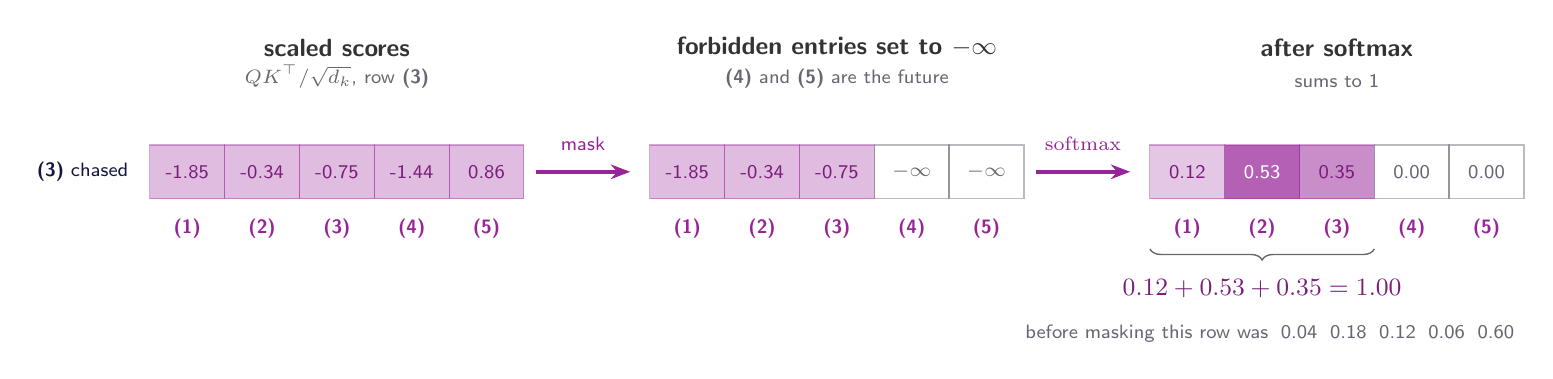
\begin{tikzpicture}[
    every node/.style={font=\sffamily},
    live/.style={draw=c2, draw opacity=0.4, line width=0.4pt},
    inert/.style={draw=labelcolor, draw opacity=0.45, line width=0.5pt},
    num/.style={font=\sffamily\scriptsize, text=c2!80!black},
    dead/.style={font=\sffamily\scriptsize, text=labelcolor},
    title/.style={font=\sffamily\small\bfseries, text=axiscolor, anchor=south},
    subtitle/.style={font=\sffamily\scriptsize, text=labelcolor, anchor=south},
    collab/.style={font=\sffamily\scriptsize, text=c2, anchor=north},
    arr/.style={-{Stealth[length=7pt]}, line width=1.3pt, c2},
    arrlab/.style={font=\sffamily\scriptsize, text=c2, anchor=south},
    note/.style={font=\sffamily\scriptsize, text=labelcolor, anchor=north},
]

% ---------------------------------------------------------- (a) scaled scores
\begin{scope}[shift={(0,0)}]
  \node[title]    at (2.375, 1.00) {scaled scores};
  \node[subtitle] at (2.375, 0.60) {$QK^{\top}/\sqrt{d_k}$, row \textbf{(3)}};
  \foreach \v [count=\c from 0] in {-1.85, -0.34, -0.75, -1.44, 0.86} {
    \fill[c2, opacity=0.30] (\c*\cw, -\ch) rectangle ++(\cw, \ch);
    \draw[live]             (\c*\cw, -\ch) rectangle ++(\cw, \ch);
    \node[num] at (\c*\cw+0.475, -0.34) {\v};
  }
\end{scope}

% ---------------------------------------------------------- (b) masked scores
\begin{scope}[shift={(\pb,0)}]
  \node[title]    at (2.375, 1.00) {forbidden entries set to $-\infty$};
  \node[subtitle] at (2.375, 0.60) {\textbf{(4)} and \textbf{(5)} are the future};
  \foreach \v/\s [count=\c from 0] in
      {-1.85/1, -0.34/1, -0.75/1, {$-\infty$}/0, {$-\infty$}/0} {
    \ifnum\s=1
      \fill[c2, opacity=0.30] (\c*\cw, -\ch) rectangle ++(\cw, \ch);
      \draw[live]             (\c*\cw, -\ch) rectangle ++(\cw, \ch);
      \node[num] at (\c*\cw+0.475, -0.34) {\v};
    \else
      \draw[inert] (\c*\cw, -\ch) rectangle ++(\cw, \ch);
      \node[dead] at (\c*\cw+0.475, -0.34) {\v};
    \fi
  }
\end{scope}

% ---------------------------------------------------------- (c) after softmax
\begin{scope}[shift={(\pc,0)}]
  \node[title]    at (2.375, 1.00) {after softmax};
  \node[subtitle] at (2.375, 0.60) {sums to 1};
  \foreach \v/\s [count=\c from 0] in
      {0.12/1, 0.53/1, 0.35/1, 0.00/0, 0.00/0} {
    \ifnum\s=1
      \pgfmathsetmacro{\op}{0.12 + 1.15*\v}
      \fill[c2, opacity=\op] (\c*\cw, -\ch) rectangle ++(\cw, \ch);
      \draw[live]            (\c*\cw, -\ch) rectangle ++(\cw, \ch);
      % dark fills need light numerals
      \pgfmathsetmacro{\vv}{\v}
      \ifdim\vv pt>0.35pt \colorlet{celltext}{white}
      \else \colorlet{celltext}{c2!80!black}\fi
      \node[font=\sffamily\scriptsize, text=celltext]
          at (\c*\cw+0.475, -0.34) {\v};
    \else
      \draw[inert] (\c*\cw, -\ch) rectangle ++(\cw, \ch);
      \node[dead] at (\c*\cw+0.475, -0.34) {\v};
    \fi
  }
  % the three survivors still make a whole distribution
  \draw[decorate, decoration={brace, mirror, amplitude=4pt},
        draw=labelcolor, line width=0.5pt] (0, -1.32) -- (3*\cw, -1.32);
  \node[note, font=\sffamily\small, text=c2!80!black] at (1.425, -1.58)
      {$0.12 + 0.53 + 0.35 = 1.00$};
\end{scope}

% ---------------------------------------------------------- column labels
\foreach \p [count=\c from 0] in {1,2,3,4,5} {
  \foreach \px in {0, \pb, \pc} {
    \node[collab] at (\px+\c*\cw+0.475, -0.82) {\textbf{(\p)}};
  }
}

% ---------------------------------------------------------- row label
\node[font=\sffamily\scriptsize, text=c1, anchor=east] at (-0.15, -0.34)
    {\textbf{(3)} chased};

% ---------------------------------------------------------- operators
\draw[arr] (4.90, -0.34) -- (6.10, -0.34);
\node[arrlab] at (5.50, -0.20) {mask};

\draw[arr] (11.25, -0.34) -- (12.45, -0.34);
\node[arrlab] at (11.85, -0.20) {$\operatorname{softmax}$};

% ---------------------------------------------------------- the contrast
\node[note, anchor=north east] at (17.45, -2.16)
    {before masking this row was\; 0.04\; 0.18\; 0.12\; 0.06\; 0.60};

\end{tikzpicture}
\end{document}
